\thispagestyle{empty}	% Pour éviter d'avoir un en-tête et un pied de page sur la page couverture

\includegraphics[width=5cm]{../figures/logoUlaval.jpg}	% Pour inclure le logo (on précise la largeur de l'image)
\hspace{4.5cm}

\includegraphics[width=7cm]{../figures/norlab_logo_acronym_dark.png}
\vspace{1cm}	% Espacement vertical

\begin{center}	% On centre le texte
{\huge \textbf{\ Marmotte \\ HD2 Robot platform \\ Technical Document}}\\ % \huge fait que le texte est gros, \bf fait que le texte est gras
\large
\vspace{1cm}
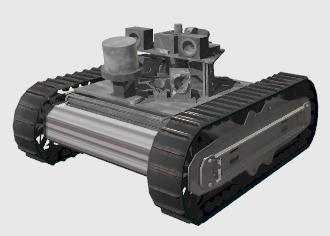
\includegraphics[width=5cm]{../figures/marmotteCAD1.png}
\vspace{1cm}

Presented to NORLab for SubT \\ DARPA competition


\vspace{4cm}
by \\ 
Nicolas Antonucci \\
Electrical engineering intern at Norlab

\vfill	% On va jusqu'au bas de la page avant de mettre le texte ci-dessous

%\today
\text{Summer 2021 project}

\pagebreak
\end{center}